\chapter{Systemidentifikation im Zeitbereich}
Systemidentifikation im Zeitbereich heißt, ein Modell und den zugehörigen 
Parametersatz zu finden, welches den zeitlichen Verlauf möglichst gut 
approximiert. Grundlegend ist hier zwischen der Systemidentifikation und der 
Parameteridentifikation zu unterscheiden. Systemidentifikation bedeutet, dass 
auch das Modell als unbekannt angenommen wird und die gesamte Struktur aus den 
Messdaten geschätzt wird, wie hier mit der Matrix-LSQ. Bei der 
Parameteridentifikation hingegen ist ein flugmechanisches Modell bekannt, in 
dem Parameter gesucht werden (vgl. LSQ).

\section{\textit{Least Squares}-Methode}
In diesem Kapitel wird die Methode der kleinsten Fehlerquadrate (\textit{Least Squares}, LSQ) vorgestellt.
Eine der Kernaufgaben vieler Ingenieure besteht darin, einen belastbaren Zusammenhang zwischen gemessenen Werten zu finden. 
Diese Zusammenhänge können näherungsweise durch folgendes lineares Modell beschrieben werden:  
\begin{equation}
    \mathbf{z} = \mathbf{H}\cdot \mathbf{x}+\mathbf{v}
\end{equation}
mit 
\begin{align}
	\begin{split}
		\text{Messvektor: } &\dim{(\mathbf{z})} = m\times 1\\
		\text{bekannte Matrix: } &\dim{(\mathbf{H})} = m\times n\\
		\text{unbekannter Rauschterm: } &\dim{(\mathbf{v})} = m\times1\\
		\text{unbekannter Parametervektor: } &\dim{(\mathbf{x})} = n\times 1
		\nonumber
	\end{split}
\end{align}

Die LSQ-Methode kann beispielsweise verwendet werden, um die Schätzung von Modellparametern im Rahmen der 
Systemidentifikation durchzuführen. Gesucht ist dabei ein Schätzwert 
$\mathbf{\hat{x}}$ für den Parametervektor. Der Restfehlervektor 
$\mathbf{e}$ lautet:
\begin{equation}
    \mathbf{e} = \mathbf{z} - \mathbf{H}\cdot \hat{\mathbf{x}} \\
\end{equation}

Die Idee besteht darin, einen Wert für $\mathbf{\hat{x}}$ zu finden, der die 
Norm des quadrierten Restfehlervektors minimiert. Das 
quadratische Zielfunktional $J$ ist gegeben durch: 
\begin{align}
   \begin{split}
     J &= \frac{1}{2} \cdot \mathbf{e}^{T} \cdot \mathbf{e} \\
     &= \frac{1}{2} \cdot {(\mathbf{z}- \mathbf{H}\mathbf{\hat{x}})}^{T}\cdot(\mathbf{z}- \mathbf{H}\mathbf{\hat{x}}) \\
     &= \frac{1}{2} \cdot (\mathbf{z}^{T} -\mathbf{\hat{x}}^{T}\mathbf{H}^{T})\cdot(\mathbf{z}- \mathbf{H}\mathbf{\hat{x}}) \\
     &= \frac{1}{2} \cdot \mathbf{z}^{T}\mathbf{z} - \mathbf{z}^{T}\mathbf{H}\mathbf{\hat{x}} + \frac{1}{2}\cdot 
     {\mathbf{\hat{x}}}^{T}\mathbf{A}\mathbf{\hat{x}}  \\
   \end{split}
\end{align}
mit $\mathbf{A} = \mathbf{H}^{T} \mathbf{H}$. Die Lösung des Minimierungsproblems lautet dann:
\begin{equation}
    \hat{\mathbf{x}}= {(\mathbf{H}^{T} \mathbf{H})}^{-1} \cdot \mathbf{H}^{T} \mathbf{z} 
    \label{eq:minProblemLoesung}
\end{equation}


\subsection{Schätzung der Parameter mit dem LSQ-Verfahren} 

Die Zustandsraumdarstellung \eqref{eq:laengsbewegung} liefert folgende Gleichungen: 

\begin{align}
	\Delta\dot \alpha-q &=  \frac{Z_{\alpha}\Delta\alpha}{V_0} + \frac{Z_{\nu}\Delta V_{A}}{V_0} + 
	\frac{Z_{\eta}\Delta\eta}{V_0} - \frac{X_{\delta_F}\sin{(\alpha_0)}\cdot\Delta\delta_F}{V_0}\\
	\dot q &= M_{\alpha}\Delta\alpha + M_q q + M_{\nu}\Delta V_A + M_{\eta}\Delta\eta + M{\delta_F}\Delta\delta_F\\
	\Delta\dot V_A &= X_{\alpha}\Delta\alpha +  X_{\nu}\Delta V_A + X_{\eta}\Delta\eta + 
	X_{\delta_F}\cos{(\alpha_0)}\cdot\Delta\delta_F \\
	\Delta \dot \gamma &= \frac{- Z_{\alpha}\Delta\alpha}{V_0} + \frac{- Z_{\nu}\Delta V_{A}}{V_0} + 
	\frac{-Z_{\eta}\Delta\eta}{V_0} + \frac{X_{\delta F}\sin{(\alpha_0)}\cdot\Delta\delta_F}{V_0}
\end{align}
	
Diese können zu einem linearen Gleichungssystem umgeformt werden: 
\begin{equation}
    \mathbf{z}_{L}= \mathbf{H}_{L}\cdot \mathbf{x} + \mathbf{v}
\end{equation}

Die einzelnen Vektoren und Matrizen lauten:
\setcounter{MaxMatrixCols}{15}
\begin{equation}
	\mathbf{z}_{L} = (\Delta\dot \alpha-q \;\; \dot q \;\; \Delta\dot V_A)^T
\end{equation}

\begin{equation}
	 \mathbf{H}_{L} = \begin{pmatrix}
		0&0&0& \frac{-\sin{(\alpha_0)}\cdot\Delta\delta_F}{V_0} & \frac{\Delta\alpha}{V_0}& \frac{\Delta V_A}{V_0} & 
		\frac{\Delta\eta}{V_0} &0&0&0&0&0   \\
		0&0&0&0&0&0&0 &\Delta\alpha & q & \Delta V_A & \Delta\eta & \Delta\delta_F \\
		\Delta\alpha &  \Delta V_A & \Delta\eta & \cos{(\alpha_0)}\cdot\Delta\delta_F &0&0&0&0&0&0&0&0 
	\end{pmatrix}
\end{equation}

\begin{equation}
	\mathbf{x} = (X_{\alpha}\; 
	X_{\nu}\;
	X_{\eta}\;
	X_{\delta_F}\; 
	Z_{\alpha}\; 
	Z_{\nu}\;
	Z_{\eta}\;
	M_{\alpha}\;
	M_{q}\;
	M_{\nu}\;
	M_{\eta}\;
	M_{\delta_F})^T \\
\end{equation}  
Wie schon in dem letzten Abschnitt erwähnt, wird es nach einem geschätzten Paramertervektor $\mathbf{\hat{x}}$ gesucht, der 
die Norm des quadrierten Restfehlervektors $ \mathbf{e} = \mathbf{z} - \mathbf{H}\cdot \mathbf{\hat{x}}$ minimiert. Die 
Lösung ist laut \cref{eq:minProblemLoesung}
\begin{equation}
    \hat{\mathbf{x}}= {({\mathbf{H}_L}^{T} {\mathbf{H}_L})}^{-1} \cdot {\mathbf{H}_L}^{T} \mathbf{z}_L 
\end{equation}



\section{Matrix-LSQ-Methode}

Bei der Matrix-LSQ-Methode werden, im Gegensatz zur klassischen LSQ-Schätzung, sowohl die Systemmatrix $ \mathbf{A} $ als 
auch die Eingangsmatrix $ \mathbf{B} $ als unbekannt angesehen. Es handelt sich somit um eine Systemidentifikation im 
eigentlichen Sinn, da keine flugmechanischen Modelle verwendet werden.

\subsection{Modellgleichung}

Die Messdaten der Eingänge $\mathbf{u}$, des Zustands  $\mathbf{x}$ und der Zustandsableitung $\dot{\mathbf{x}}$ werden in 
die Form von \cref{eq:matrixLSQ} gebracht. 

\begin{equation}
    \underbrace{\begin{pmatrix}
        \dot{x}_1^T \\
        . \\
        . \\
        \dot{x}_n^T 
    \end{pmatrix}}_{\mathbf{z}} =
    \underbrace{\begin{pmatrix}
        x_{1}^T& u_{1}^T \\
        . & .  \\
        . & .  \\
        x_{n}^T & u_{n}^T \\
    \end{pmatrix}}_{\mathbf{H}}
    \underbrace{\begin{pmatrix}
        \mathbf{A}^T \\
        \mathbf{B}^T
    \end{pmatrix}}_{\hat{\mathbf{x}}} +
    \begin{pmatrix}
        v_1^T \\
        . \\
        . \\
        v_n^T
    \end{pmatrix}
	\label{eq:matrixLSQ}
\end{equation}

\begin{tabular}[\textwidth]{l l}

$\mathbf{z}$ & Messmatrix \\
$\mathbf{H}$ & Modellmatrix \\
$\hat{\mathbf{x}}$ & Schätzwertmatrix \\
$\mathbf{v}$ & Störgrößenmatrix \\
$n$ & Anzahl der Zeitschritte \\
\end{tabular}

Die Dimension der Systemmatrix und der Eingangsmatrix werden von den Dimensionen von $\mathbf{u}$,  $\mathbf{x}$ und 
$\dot{\mathbf{x}}$ vorgegeben. Hier liegt auch der Nachteil der Matrix-LSQ-Methode. Es ist nicht möglich die einzelnen 
Parameter innerhalb der Matrizen zu beeinflussen oder Wertebereiche vorzugeben.


\subsection{Schätzgleichung}

Nach der Herleitung in \cite{Mandry2021} ergibt sich die Schätzgleichung zu:

\begin{equation*}
    \hat{\mathbf{x}} = (\mathbf{H}^T \mathbf{H})^{-1}\mathbf{H}^T\mathbf{z}
\end{equation*}

Besonders hervorzuheben ist hier die Inversion der Matrix $\mathbf{H}^T \mathbf{H}$. Es handelt sich dabei um eine Matrix der 
Dimension $ (\dim{(\mathbf{x})}+\dim{(\mathbf{u})}) \times (\dim{(\mathbf{x})}+\dim{(\mathbf{u})}) $. In dieser Arbeit 
bedeutet das konkret eine Dimension $ 6 \times 6 $, womit der Rechenaufwand für 
die - für große Matrizen aufwändige - Inversion klein bleibt.
 
\section{Ergebnisse}
 
Anschließend werden die Ergebnisse in diesem Kapitel kurz vorgestellt.

Nach der Schätzung der Einträge der Matrizen $\mathbf{A}$ und $\mathbf{B}$ wird das Anfangswertproblem 
\eqref{eq:laengsbewegung} im gesamten Zeitintervall gelöst. Bei allen Simulationen sind die Filterparametern wie in 
\cref{section:filterung} gewählt.

In \cref{fig:Ergebnisse_zmlsq} wird die Lösung anhand des Matrix-LSQ-Verfahrens dargestellt. Die geschätzten Matrizen 
$\mathbf{A_L}$ und $\mathbf{B_L}$ lauten: 
\begin{equation}
 	\mathbf{A_L}\mathbf = \begin{pmatrix}
 		-0.1940 & 0.005 & -0.0002 & -0.0540 \\
 		-38.9899 & -12.8888 & 0.3632 & -4.2686 \\
 		-6.1506 & -0.1501 & -0.0589 & -5.0107 \\
 		0.4433 & 0.0427 & 0.0023 & 0.0818
 	\end{pmatrix} \;\;\; , \;\;\;
 	\mathbf{A} = \begin{pmatrix}
		\frac{Z_\alpha}{V_0} & 1 & \frac{Z_V}{V_0} & 0\\
		M_\alpha & M_q & M_V & 0\\
		X_\alpha & 0 & X_V & -g\\
		-\frac{Z_\alpha}{V_0} & 0 & -\frac{Z_V}{V_0} & 0\\
	\end{pmatrix}
	\nonumber
\end{equation}

\begin{equation}
 	 \mathbf{B_L} = \begin{pmatrix}
 		-0.0267 & -0.0164 \\ 
 		-26.1377 & -12.9651 \\
 		-0.7414 & 4.6092 \\
 		0.0477 & -0.1328
 	\end{pmatrix}  \;\;\; , \;\;\;
 	\mathbf{B}= \begin{pmatrix}
		\frac{Z_\eta}{V_0} & -\frac{X_{\delta_F}}{V_0} \sin{(\alpha_0)}\\
		M_\eta & M_{\delta F}\\
		X_\eta & X_{\delta F} \cos{(\alpha_0)}\\
		-\frac{Z_\eta}{V_0} & \frac{X_{\delta_F}}{V_0} \sin{(\alpha_0)}\\
	\end{pmatrix}
 \nonumber
\end{equation}

Die Ergebnisse in \cref{fig:Ergebnisse_zmlsq} zeigen eine relativ präzise Approximation, das Modell liefert vor allem für 
Anstellwinkel und Geschwindigkeit gute Ergebnisse. Auch die Ergebnisse für $ q $ und den Bahnwinkel sind sinnvoll, durch die 
wenig aussagekräftigen Messdaten aber schwer zu vergleichen. Allerdings weist das Ergebnis in flugmechanischer Hinsicht 
Abweichungen in System- und Eingangsmatrix auf. Die Beträge der Einträge der ersten und vierten Zeile von $\mathbf{A_L}$ 
unterscheiden sich stark voneinander ($0.1940$ und $0.4433$) und ($0.0002$ und $0.0023$), obwohl diese beim ersten, dritten 
und vierten Eintrag aufgrund $\Delta \gamma = \Delta \theta - \Delta \alpha$ gleich sein sollten. Eine starke Abweichung ist 
auch zwischen den vierten Spalten der Matrizen $A_L$ und $A$ zu sehen.

%\todo{warum schlechte Ergebnisse? : Adam : ich weiß nicht warum?}
\begin{figure}[h!]
	\centering
	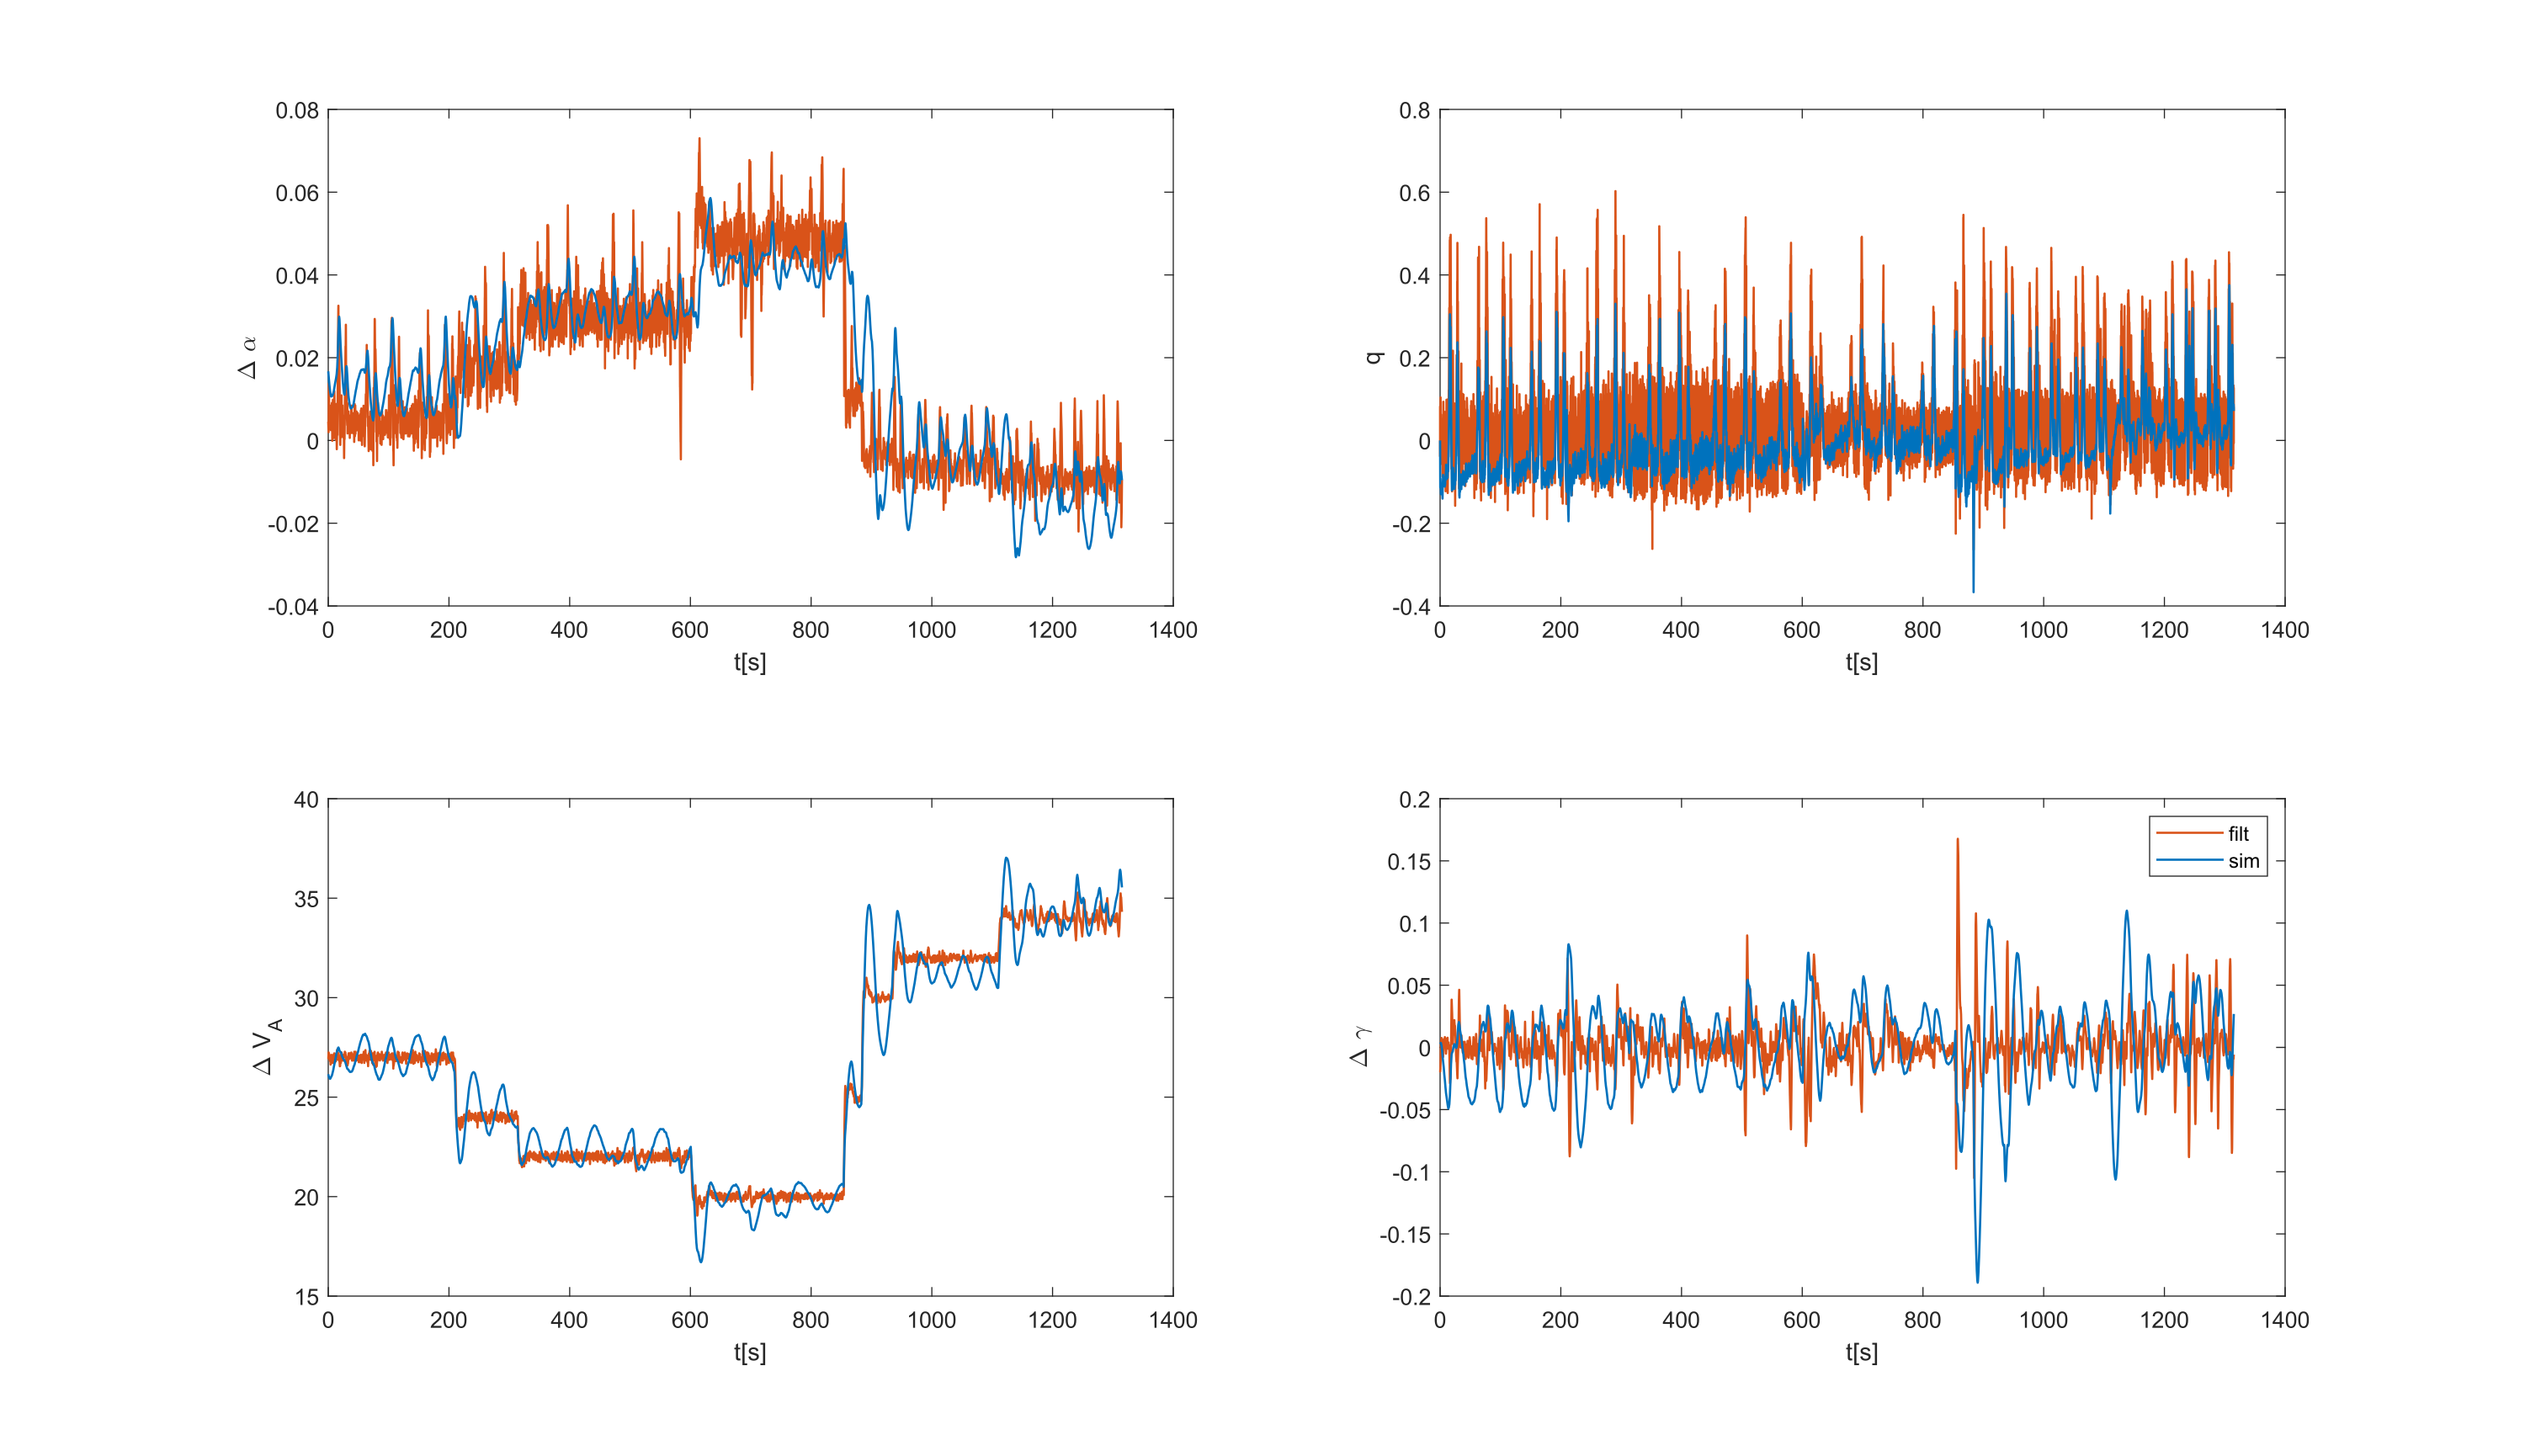
\includegraphics[trim=100 0 100 0,clip,width=1\linewidth]{LS.png}
	\caption{Ergebnisse anhand des Matrix-LSQ-Verfahrens}
    \label{fig:Ergebnisse_zmlsq}
\end{figure}

\cref{fig:Ergebnisse_zlsq} zeigt die Lösung anhand des LSQ-Verfahrens. Die Methode liefert kein sinnvolles Ergebnisse. Die 
Simulation ist nicht stabil.

 \begin{figure}[h!]
	\centering
	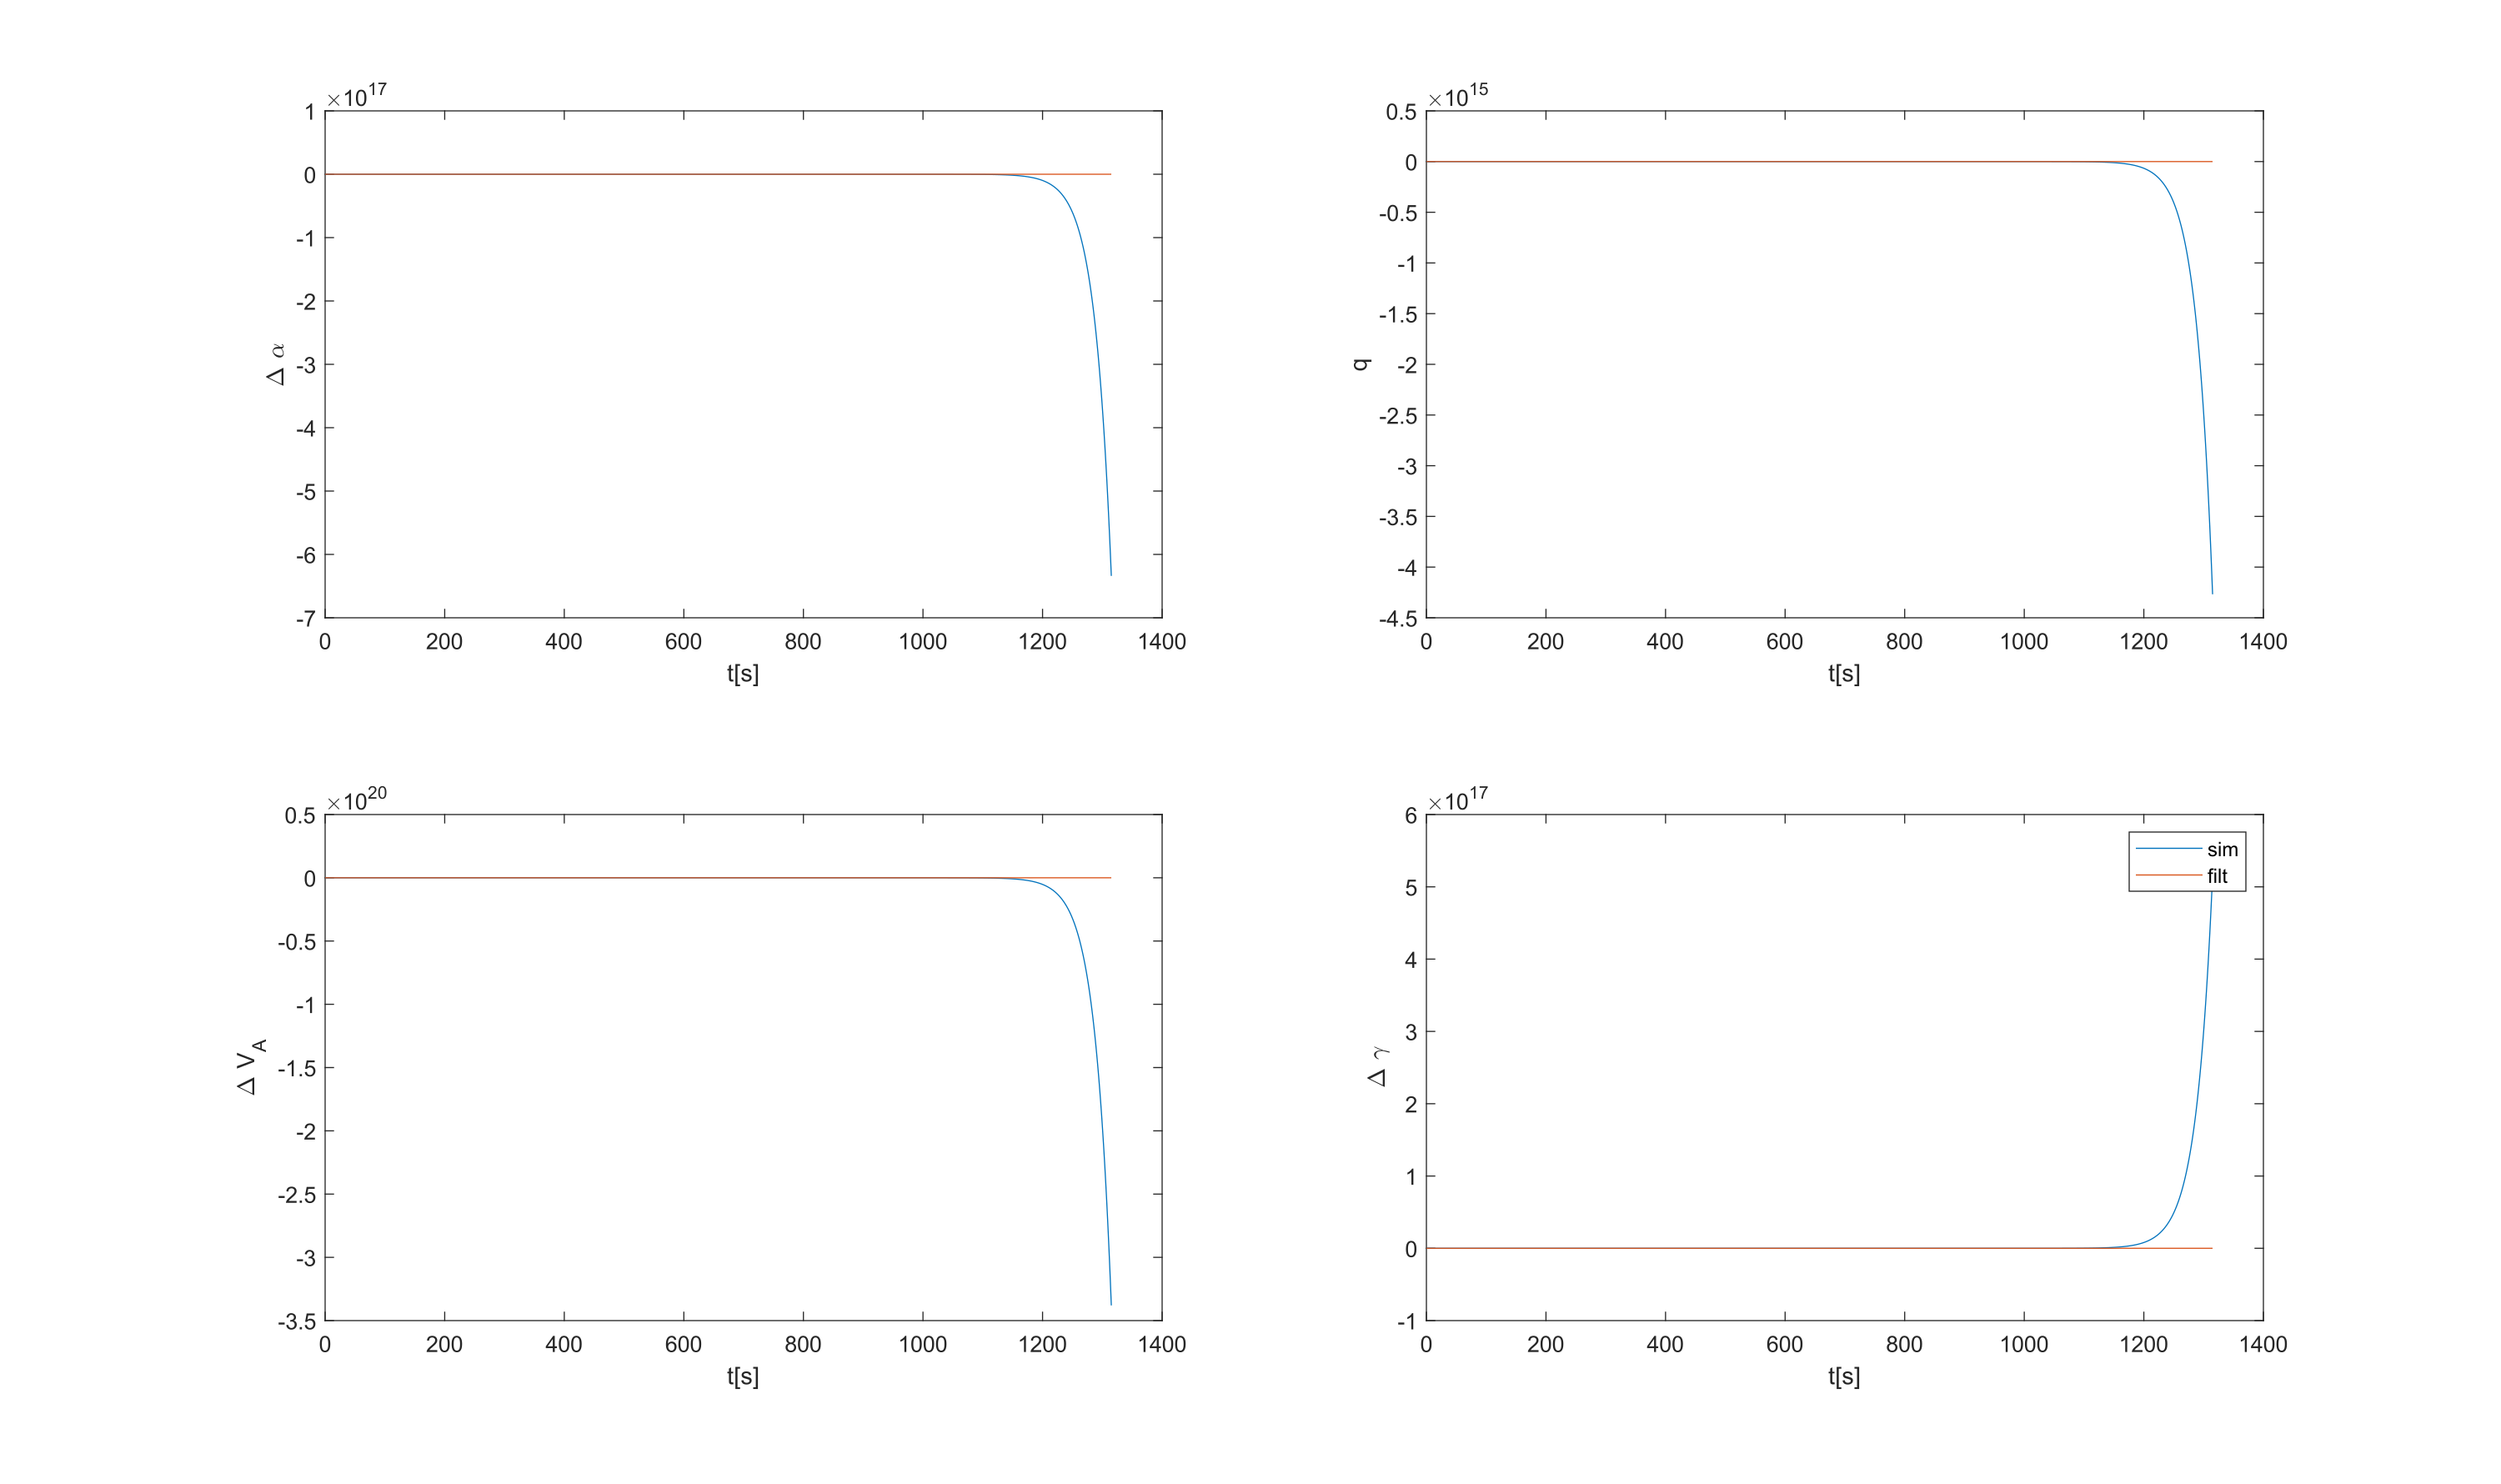
\includegraphics[trim=100 0 100 0,clip,width=1\linewidth]{LS_LSQ.png}
	\caption{Ergebnisse anhand des LSQ-Verfahrens}
     \label{fig:Ergebnisse_zlsq} 
\end{figure}


\section{Interpretation}

%Die wesentliche Erkenntnis der Analyse im Zeitbereich ist, dass es nicht möglich ist, die Parameter des linearen Modells für 
%die Längsbewegung so zu bestimmen, dass eine stabile Simulation möglich ist.
%
%Eine Interpretation dafür ist, dass mithilfe der Matrix-LSQ Effekte übertragen werden, die vom linearen Modell 
%vernachlässigt werden. Die in Kap. \ref{chapter:Modell} beschriebenen Vereinfachungen sind hier ein guter Ansatz. Besonders 
%ist es möglich, dass der Wind und der Auftrieb durch die Nickrate eine relevante Rolle spielt. 
%%Gerade die Elemente A[1,4] und A[2,4] sprechen dafür, weil durch diese der Bahnwinkel auf die Änderung des Anstellwinkels 
%%übertragen wird. 
%
%Dass Element $\mathbf{A}_L[1,4]$ nicht null ist spricht für einen Einfluss des Windes, weil somit $\Delta \gamma = \Delta 
%\theta- \Delta \alpha$ nicht mehr gilt. Der Bahnwinkel hat somit einen Einfluss auf den Anstellwinkel.
%
%Eine weitere Untersuchung und eine Betrachtung der Bedingungen beim Flugversuch sind hier notwendig, um eine fundierte 
%Aussage zu treffen.

Die wesentliche Erkenntnis der Analyse im Zeitbereich ist, dass es mit der LSQ-Methode nicht möglich ist, die Parameter des 
linearen Modells für die Längsbewegung so zu bestimmen, dass eine stabile Simulation möglich ist. Mit der Matrix-LSQ-Methode 
lassen sich Matrizen $ A_L $ und $ B_L $ finden, mit denen die Messdaten angenähert werden können. Jedoch treten hier 
Abweichungen von dem ursprünglichen Modell auf.\par
Eine mögliche Erklärung dafür ist, dass die Einträge der mit Matrix-LSQ identifizierten Systemmatrix ungleich $ 0 $ eine 
Übertragung von Effekten ermöglichen, zu der das ursprüngliche Modell nicht in der Lage ist. Die in \cref{chapter:Modell} 
beschriebenen Vereinfachungen sind hier ein guter Ansatz. Besonders ist es möglich, dass der Wind und der Auftrieb durch die 
Nickrate eine relevante Rolle spielen. 
%Gerade die Elemente A[1,4] und A[2,4] sprechen dafür, weil durch diese der Bahnwinkel auf die Änderung des Anstellwinkels 
%übertragen wird. 

Die Unterschiede in der ersten und vierten Zeile der Systemmatrix sprechen für einen Einfluss des Windes, weil somit $\Delta 
\gamma = \Delta \theta - \Delta \alpha$ nicht mehr gilt.\footnote{Der Bahnwinkel hat somit einen Einfluss auf den 
Anstellwinkel.}
Eine weitere Untersuchung und eine Betrachtung der Bedingungen beim Flugversuch sind hier notwendig, um eine fundierte 
Aussage treffen zu können.
